\section{Arjun Yuda Firwanda (1174008)}
\subsection{Pengertian}
Sistem Informasi Geografis merupakan sistem informasi yang secara khusus mengelola data yang memiliki spasial atau keruangan.

Secara ringkasnya sistem informasi geografis merupakan sistem komputer yang memiliki kemampuan untuk membangun, menyimpan, mengelola dan menampilkan informasi bereferensi geografis, contohnya sebuah data yang diidentifikasi menurut lokasinya.

Pengertian Sistem Informasi Geografis merupakan gabungan dari tiga unsur pokok.
\begin{itemize}
	\item Sistem merupakan sekumpulan objek.
	\item Sistem Informasi merupakan sistem antara manusia dan mesin untuk menyajikan informasi untuk mendukung suatu fungsi operasi, manajemen dan pengambilan keputusan.
	\item Geografi  merupakan pengertian yang mengenai tempat-tempat yang terletak di permukaan bumi dan informasi mengenai keterangan dan posisi yang terdapat di permukaan bumi.
\end{itemize}

\subsection{Sejarah}
Awal dikenalnya Sistem Informasi Geografis (Geogragis Informastion System) tidak lepas dari perkembangan dalam bidang teknologi. Pada awal 1960-an perkembangan teknologi digunakan untuk bidang diluar militer. Pada ahli meterologi, geologi dan geofisika mulai menggunakan komputer dalam pembuatan peta.

Tahun 1963 di Kanada muncul CGIS (Canada Geographic Information System) dan selanjutnya menjadi GIS pertama di dunia. Dua tahun kemudian di Amerika Serikat beroperasi sistem bernama MIDAS yang digunakan untuk memproses data-data sumber daya alam.

\subsection{Koordinat}
Sistem Koordinat, osisi suatu titik biasanya dapat dinyatakan dengan koordinat yang mengacu pada suatu sistem koordinat tertentu.

\begin{itemize}
	\item Lokasi Titik Nol dari Sistem Koordinat
Posisi suatu titik di permukaan bumi umumnya ditetapkan dalam/terhadap suatu sistem koordinat terestris. Titik nol dari sistem koordinat terestris ini dapat berlokasi di titik pusat massa bumi (sistem koordinat geosentrik), maupun di salah satu titik di permukaan bumi (sistem koordinat toposentrik).  
	\item Orientasi dari Sumbu-sumbu Koordinat
Posisi tiga-dimensi suatu titik di permukaan bumi umumnya dinyatakan dalam suatu sistem koordinat geosentrik. Tergantung dari parameter-parameter pendefinisi koordinat yang digunakan. Ada dua sistem koordinat yang umum digunakan, yaitu sistem koordinat Kartesian (X,Y,Z) dan sistem koordinat Geodetik (L,B,h).
\end{itemize}


\subsection{Data Geospasial}
Data geospasial adalah kumpulan fakta yang berupa informasi tentang ruang kebumian (geospasial) yang menunjukan lokasi atau posisi dari suatu tempat atau objek yang direpresentasikan pada sebuah garis titik koordinat. Data geospasial dibagi menjadi 2 yaitu:

\begin{enumerate}
	\item Data Vector
Dalam bentuk data vector bagian objek dibumi ditampilkan sebagai kumpulan titik , garis dan polygon dimana sekumpulan tiitik yang saling terhubung akan membentuk garis dan garis yang saling terhubung antara titik awal dan titik akhir dengan nilai koordinat ynag sama akan membentuk polygon . Data vector dibagi menjadi 2 yaitu:

	\begin{itemize}
		\item Culture, memaparkan atau menampilkan data geospasial yang disertai dengan nama atribut atau memberikan keterangan atas nama dari objek di bumi. Contohnya nama dari suatu Negara, indicator batas air (keterangan kedalaman air laut), nama provinsi, daerah, wilayah dsb.
		\item Physical, memaparkan atau menampilkan data geospasial mengenai bentuk fisiknya atau gambaran tentang objek-objek alam yang ada dibumi. Contohnya gambaran laut, garis pantai, terumbu karang, danau dsb.
	\end{itemize}

	\item Data Raster, dapat menampilkan permukaan bumi seperti bentuk aslinya atau seperti dalam peta asli yang terlihat jelas dari setiap objek dengan keadaan alamnya. Data raster dibentuk agar menampilkan objek berupa elemen matriks atau grid, yang merepresentasikan objek dari data geospasial mengenai batas-batas yang berubah, ketinggian tanah.
\end{enumerate}

\subsection{Link}
\href{https://www.youtube.com/watch?v=HGscljVrxrE&feature=youtu.be}{Cek Di Youtubeku}

\subsection{Plagiarism}
\begin{figure}[Cek Plagiat]
	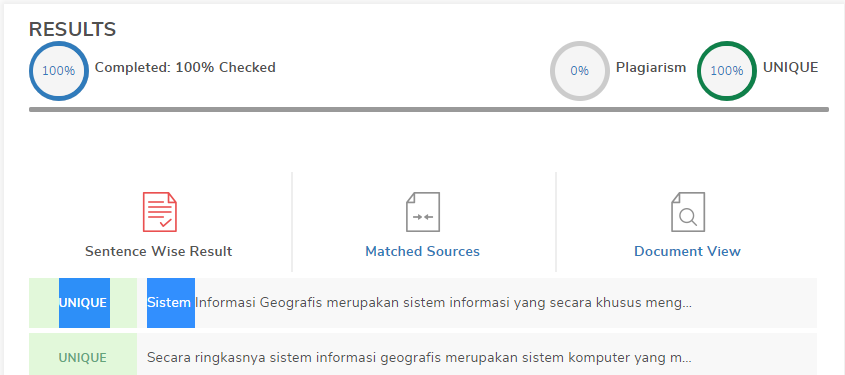
\includegraphics[width=4cm]{figures/1174008/pelagiat.png}
	\centering
	\caption{Cek Plagiat.}
\end{figure}
